% Working manuscript for methodological discussion; not submission-ready.
% Compile from this directory: pdflatex, bibtex, pdflatex, pdflatex.
\documentclass[11pt]{article}
\usepackage[margin=1in]{geometry}
\usepackage[T1]{fontenc}
\usepackage{lmodern}
\usepackage{amsmath,amssymb,booktabs,graphicx}
\usepackage{float}
\usepackage[authoryear,round]{natbib}
\usepackage{microtype}
\usepackage[hidelinks]{hyperref}
\usepackage{xcolor}
\newcommand{\E}{\mathrm{E}}
\newcommand{\I}{\mathbf{1}}
\newcommand{\Hist}{\mathcal{H}}
\newcommand{\Risk}{\mathcal{R}}
\title{Temporal Exponential Random Graph Models and Relational Hyperevent Models as Benchmarks for Forecasting Directed Group Interactions}
\author{Moses Boudourides\\School of Professional Studies, Northwestern University\\\texttt{Moses.Boudourides@northwestern.edu}}
\date{Working manuscript --- 30 October 2026}

\begin{document}
\maketitle

\begin{abstract}
A directed group interaction has a temporal object that is lost in a static projection: at time $t$, one sender addresses a particular receiver set. This manuscript develops a reproducible temporal extension of a missingness-centred benchmark for directed link and hyperlink prediction. The event-level component uses audited Enron email records, an actor universe selected only before the forecast origin, four expanding 2001 origins, and a relational hyperevent model (RHEM) for receiver-set choice conditional on the observed sender and receiver-set size. It compares a dyadic-history specification with a group-augmented specification that adds exact receiver-set and receiver-pair repetition. In the primary source-record representation, the group terms improve sampled-risk-set discrimination for the 108 multiple-receiver test events. The direction of the log-score contrast changes, however, when identical timestamp--sender--receiver-set records are collapsed, although rank-oriented measures still improve. This representation sensitivity, together with abundant timestamp ties, prevents a substantive higher-order claim. The manuscript therefore contributes an audited temporal directed-hyperevent workflow and a clearly bounded feasibility result rather than a final claim of RHEM superiority. A short btergm exercise is retained as a dyadic temporal-ERGM companion; its two-transition panels are insufficient for event-level forecasting or coefficient interpretation. The central methodological conclusion is that temporal dyadic and temporal hyperevent models answer different forecasting questions and must be evaluated on explicitly defined histories, risk sets, and event representations.
\end{abstract}

\noindent\textbf{Keywords:} relational hyperevent models; temporal networks; directed hypergraphs; temporal ERGMs; btergm; receiver-set choice; Enron email

\section{Introduction}\label{sec:introduction}

The first manuscript in this project distinguishes recorded directed group events, their dyadic footprints, and groups reconstructed algebraically from a static projection. That distinction becomes sharper once records are dated. A temporal directed group event is not merely a static rectangle observed at a time label. It is an action: a sender selects a receiver set at a particular instant, against a risk set determined by the actor universe and the event history. A static ERGM score for a projected arc does not, by itself, estimate the probability that a sender selects a particular group next.

Relational event models represent directed actions as event sequences \citep{butts2008}. Relational hyperevent models (RHEMs) extend that framework from one receiver to a set of receivers and allow covariates that are functions of the entire ordered hyperedge \citep{lernerLomi2023}. This makes RHEMs the natural event-level counterpart to a temporal ERGM (TERGM) or btergm model, which represents evolution of a dyadic network. The models are complementary rather than interchangeable: a TERGM asks about the distribution of a network panel conditional on earlier panels, while a RHEM can rank a receiver set conditional on a sender, time, and event history.

This working manuscript makes that distinction operational. Its primary analysis is an audited, rolling-origin RHEM exercise on a temporal directed Enron email projection. It asks a deliberately narrow question: conditional on the observed sender and observed receiver-set size, does adding group-level event history improve the ranking of the observed receiver set against sampled alternatives? The answer is informative but not yet a stable scientific conclusion. The primary source-record representation shows an improvement concentrated in multiple-receiver events; a same-timestamp representation sensitivity changes the log-score conclusion. Reporting both outcomes is essential, because raw email archives contain replicated records and many simultaneous timestamps.

The manuscript also retains the previously constructed btergm ladder as a bounded dyadic companion. Its role is diagnostic: it illustrates the relationship between lagged dyadic predictors and temporal ERGM estimation, but it neither forecasts native email events nor provides a mature competitor to the RHEM. This explicit separation responds to a common scope error in temporal-network work: a good score for a projected dyad is not evidence that a model has recovered the sender and receiver set of an interaction.

\section{Temporal objects and forecasting targets}\label{sec:targets}

Let $V$ be an actor universe. A native directed group event is
\begin{equation}
 e_m=(t_m,s_m,H_m), \qquad s_m\in V, \quad \varnothing\ne H_m\subseteq V\setminus\{s_m\},
 \label{eq:event}
\end{equation}
where $t_m$ is an event time, $s_m$ is the sender, and $H_m$ is an unordered nonempty receiver set. Its directed dyadic footprint is $\{(s_m,j):j\in H_m\}$. Aggregating these footprints over time yields a directed graph, but that graph does not preserve the partition of arcs into receiver sets, the multiplicity of a receiver set, or the ordering of events.

The temporal event-level target is receiver-set choice. Conditional on the observed sender $s_m$ and cardinality $k_m=|H_m|$, define the risk set
\begin{equation}
 \Risk_m=\{J\subseteq V\setminus\{s_m\}:|J|=k_m\}.
 \label{eq:riskset}
\end{equation}
This is a conditional target. It does \emph{not} model when an email occurs, who sends it, or its recipient count. It ranks the observed $H_m$ against same-size alternatives for the given sender. Conditioning is useful here because it makes the event-level role grammar explicit and keeps the initial analysis computationally tractable. It also makes the interpretation narrower than an unconditional email forecast.

For history just before $t$, a RHEM specifies an intensity
\begin{equation}
 \lambda_\theta(s,J\mid\Hist_{t^-})=\lambda_0(t)\exp\{\theta^\top z(s,J,\Hist_{t^-})\},
 \label{eq:rhem-intensity}
\end{equation}
where $z$ can include dyadic and genuinely group-level functions of prior events. The corresponding conditional receiver-set probability is
\begin{equation}
 \Pr_\theta(H_m\mid s_m,k_m,\Hist_{t_m^-})=
 \frac{\exp\{\theta^\top z(s_m,H_m,\Hist_{t_m^-})\}}
 {\sum_{J\in\Risk_m}\exp\{\theta^\top z(s_m,J,\Hist_{t_m^-})\}}.
 \label{eq:conditional-choice}
\end{equation}
For $|V|=50$, direct enumeration becomes infeasible for larger $k_m$. We therefore use the sampled-risk-set conditional-likelihood strategy described by \citet{lernerLomi2023}: the observed receiver set is compared with a fixed number of same-size sampled non-events. The resulting score is a probability \emph{within the sampled choice set}; it is not the population probability in \eqref{eq:conditional-choice}.

A temporal ERGM instead represents a sequence of dyadic networks $Y_t$. A generic first-order formulation is
\begin{equation}
 \Pr_\theta(Y_t=y\mid Y_{t-1})\propto
 \exp\{\theta^\top g(y,Y_{t-1})\},
 \label{eq:tergm}
\end{equation}
where $g$ can contain lagged and contemporaneous network statistics \citep{hannekeEtAl2010,leifeldEtAl2018}. A lagged-only model yields conditional dyadic scores. It cannot, without a further event-generation rule, specify how a sender chooses a receiver set or how a set of arcs is bundled into a native interaction. The RHEM and the TERGM therefore occupy different levels of the temporal data-generating record.

\section{Data and temporal design}\label{sec:data}

\subsection{Audited Enron event records}

The source is the Enron email corpus \citep{klimtYang2004}, processed under the strict custodian mapping, UTC timestamp, and sender-removal rules established in the project audit. A retained native event has one mapped custodian sender and a nonempty set of mapped To/Cc recipients. Distinct source records are retained in the primary representation even if their timestamp, sender, and receiver set coincide. This preserves the project-wide source-record policy, but it makes the treatment of ties a methodological choice rather than a harmless implementation detail.

The temporal RHEM cohort uses 50 actors selected by total participation \emph{before} 1 January 2001. This origin-safe rule prevents later test events from determining the actor universe. The retained sequence runs from May 1999 through December 2001. Table~\ref{tab:design} describes the cohort, the four expanding quarterly origins, and the representation sensitivity. The primary representation contains 5,231 events, including 178 multiple-receiver events; 4,699 records occur in a timestamp tie. The test period contains 2,797 events, but only 108 have multiple receivers. The latter is the only stratum in which a receiver-set statistic can express nontrivial polyadic information, and its small size governs the strength of any conclusion.

\begin{table}[t]
\centering
\caption{Origin-safe Enron temporal event design. The 50-actor universe is ranked using sender-or-receiver participation strictly before 1 January 2001. The primary source-record representation preserves distinct projected records; the final row is an explicitly labelled representation sensitivity.}
\label{tab:design}
\small
\begin{tabular}{lrr}
\toprule
Quantity & Primary & Footprint-collapse sensitivity \\
\midrule
Actor universe & 50 & 50 \\
Pre-origin retained events & 2,434 & --- \\
Events through 2001 & 5,231 & 2,345 \\
Events with $|H|\geq2$ & 178 & 78 \\
Records in timestamp ties & 4,699 & --- \\
Identical time--sender--head records removed & 0 & 2,886 \\
2001 test choice sets & 2,797 & 1,411 \\
\bottomrule
\end{tabular}

\vspace{0.6em}
\begin{tabular}{lrr}
\toprule
Fold & Training events & Test events \\
\midrule
2001\_q1 & 2,434 & 1,014 \\
2001\_q2 & 3,448 & 883 \\
2001\_q3 & 4,331 & 269 \\
2001\_q4 & 4,600 & 631 \\
\bottomrule
\end{tabular}
\end{table}


\subsection{Risk-set, tie, and representation policies}

The Eventnet implementation \citep{eventnet2026} generates 100 requested same-size non-events per observed event using a fixed XML random seed. A singleton-recipient event has only 49 possible receivers in a 50-actor universe, so the actual candidate count may be smaller than 101. The primary run uses a deterministic increasing record-ID order within identical timestamps. Two predeclared checks use a second random seed for sampled controls and the reverse record order. These assess only two implementation choices; they do not make simultaneity substantively ordered.

A fourth run collapses identical timestamp--sender--receiver-set records after the actor universe is fixed. It removes 2,886 records and reduces the 2001 test sequence from 2,797 to 1,411 events. It is an event-representation sensitivity, not an estimate of sampling uncertainty. In particular, it deliberately answers a different question: whether repetition recorded at the same timestamp should be treated as separate event occurrences or as one footprint occurrence.

\section{Models, fitting, and evaluation}\label{sec:methods}

\subsection{History statistics and model ladder}

Eventnet updates event histories sequentially with a seven-day exponential-decay half-life. The \emph{dyadic-history} model contains square-root transformed directed dyad repetition, reciprocation, and transitive closure statistics. The \emph{group-augmented} model adds exact repetition of the sender--receiver-set event and repetition of receiver pairs. The latter two statistics cannot generally be decomposed into independent sender--receiver dyads. This is a deliberately small ladder: it tests whether a limited group-history increment changes discrimination beyond a transparent dyadic-history reference. It does not search a large menu of effects or claim a complete behavioral theory of email.

For each origin, the implementation exports the observed and sampled non-events with an \texttt{EVENT\_INTERVAL} identifier. We estimate the sampled conditional likelihood with \texttt{survival::coxph}, stratifying on this interval. Thus each stratum compares exactly one observed event with its sampled alternatives. Coefficients are estimated using only events before the test-quarter origin. During each test quarter, history statistics use events preceding the event in the declared sequence; the coefficients remain fixed. This is a one-step online ranking design, not a model that fits on held-out outcomes.

The reported performance measures are the mean conditional log score, tie-adjusted Top-1 recovery, tie-adjusted mean reciprocal rank (MRR), and mean rank. They are pooled over the four fixed quarterly folds by number of evaluated choice sets. A score difference is reported descriptively. Neither four temporal folds nor the 48--108 multi-receiver test events support a general-population confidence claim.

\subsection{Temporal-ERGM companion}

The project also contains a bounded btergm ladder estimated by maximum pseudolikelihood with temporal bootstrap intervals \citep{leifeldEtAl2018}. It uses short dyadic panels prepared before the RHEM study. Table~\ref{tab:btergm-boundary} records its appropriate evidential role. The Enron panel has only two response transitions and nonfinite higher-order fits; the EU-core panel has finite fits but no observed native receiver sets. These artifacts are useful warnings about panel definition and separation, not a completed TERGM-versus-RHEM competition.

\section{Results}\label{sec:results}

\subsection{Primary rolling receiver-set evaluation}

Table~\ref{tab:primary-rhem} reports the primary fixed-seed, source-record result. Across all 2,797 evaluated events, the group-augmented model improves the sampled conditional log score from $-1.483$ to $-1.447$ and Top-1 recovery from $0.644$ to $0.652$. The all-event aggregate is driven largely by singleton-recipient messages. In that subset, the log-score difference is essentially zero and the rank measures change little. This is consistent with the fact that the group statistics have limited additional content when $|H|=1$.

The multiple-receiver stratum yields a different pattern. On 108 test events, the group-augmented specification has a log score of $-0.943$ versus $-1.877$ for dyadic history, Top-1 recovery of $0.864$ versus $0.753$, and MRR of $0.912$ versus $0.822$. These are conditional discrimination statistics within Eventnet's sampled alternative sets. They show that, in the primary representation, repeated receiver-set and receiver-pair history can reorder candidates in a way that dyadic histories alone do not. They do not identify a stable social mechanism or an unconditional probability of a multi-recipient email.

\begin{table}[t]
\centering
\caption{Primary conditional-sender RHEM evaluation, pooled over four expanding 2001 quarters. Every event is ranked only against Eventnet-sampled receiver sets of the same observed size for the observed sender. Metrics are therefore sampled-choice-set discrimination measures, not unconditional event probabilities.}
\label{tab:primary-rhem}
\small
\begin{tabular}{llrrrrr}
\toprule
Scope & Model & Choice sets & Log score & Top-1 & MRR & Mean rank \\
\midrule
All receiver-set events & Dyadic history & 2,797 & -1.483 & 0.644 & 0.780 & 2.125 \\
All receiver-set events & Dyadic + group history & 2,797 & -1.447 & 0.652 & 0.786 & 2.226 \\
Singleton receiver & Dyadic history & 2,689 & -1.467 & 0.640 & 0.779 & 2.118 \\
Singleton receiver & Dyadic + group history & 2,689 & -1.467 & 0.644 & 0.781 & 2.252 \\
Multiple receivers & Dyadic history & 108 & -1.877 & 0.753 & 0.822 & 2.296 \\
Multiple receivers & Dyadic + group history & 108 & -0.943 & 0.864 & 0.912 & 1.602 \\
\bottomrule
\end{tabular}
\end{table}


\subsection{Sensitivity to candidate sampling, ties, and event representation}

The first three rows of Table~\ref{tab:rhem-sensitivity} retain the source-record representation. The multiple-receiver log-score increment is positive under a new sampled-control seed ($+0.581$) and under reverse ordering of tied timestamps ($+0.971$), while Top-1 and MRR increments remain positive. This establishes a limited robustness of the ranking result to these two algorithmic choices.

The representation sensitivity is more consequential. Collapsing same-timestamp identical footprints reduces the multiple-receiver test set to 48 events. The group-augmented model retains higher Top-1 and MRR in that run, but its conditional log-score contrast becomes negative ($-0.893$). Figure~\ref{fig:rhem-sensitivity} displays the conflict. A result that changes direction under a defensible record-representation policy cannot be presented as evidence that higher-order history has a stable advantage. The appropriate conclusion is narrower: the effect of group-history features is task- and representation-dependent, and the source archive's duplicate/tie semantics must be part of the estimand.

\begin{table}[t]
\centering
\caption{Sensitivity of the group-augmented minus dyadic-history comparison for multiple-receiver events. Positive log-score, Top-1, and MRR differences favor the group-augmented model; a negative mean-rank difference favors it. The final sensitivity changes the event representation itself, so it is not an uncertainty interval around the primary design.}
\label{tab:rhem-sensitivity}
\small
\begin{tabular}{lrrrrr}
\toprule
Sensitivity & Choice sets & $\Delta$ log score & $\Delta$ Top-1 & $\Delta$ MRR & $\Delta$ rank \\
\midrule
Primary: ascending order, seed 20261030 & 108 & +0.934 & +0.111 & +0.090 & -0.694 \\
Control-sampling seed 20261031 & 108 & +0.581 & +0.137 & +0.107 & -0.907 \\
Descending tied-time order & 108 & +0.971 & +0.093 & +0.080 & -0.704 \\
Collapse identical time--role footprints & 48 & -0.893 & +0.079 & +0.076 & -1.958 \\
\bottomrule
\end{tabular}
\end{table}


\begin{figure}[t]
\centering
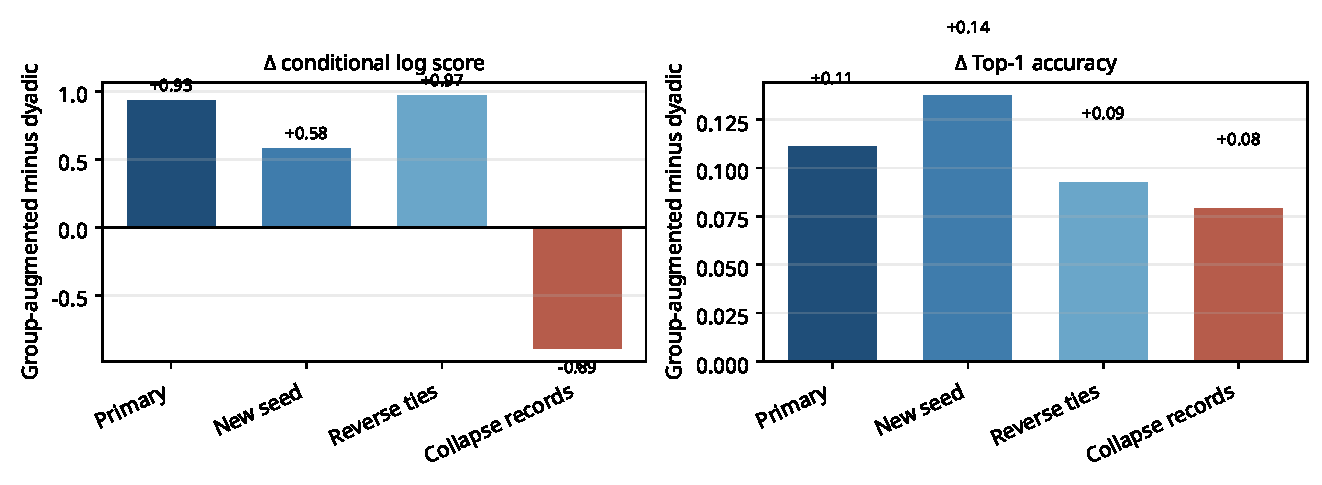
\includegraphics[width=\textwidth]{figures/figure_01_group_contrast_sensitivity.pdf}
\caption{Pooled group-augmented minus dyadic-history contrasts for multiple-receiver events. The first three columns preserve source records and vary the sampled-control seed or within-timestamp order. The final column collapses identical timestamp--sender--receiver-set footprints and is a different event representation, not a confidence interval.}
\label{fig:rhem-sensitivity}
\end{figure}

\subsection{Bounded temporal-ERGM diagnostic}

The short btergm evidence does not alter this conclusion. As Table~\ref{tab:btergm-boundary} shows, the Enron temporal panel has nonfinite higher-order MPLE fits, and the EU-core result is a two-transition dyadic check. These outcomes preclude a meaningful test of whether a temporal ERGM can match receiver-set forecasting. They instead motivate the paper's design principle: a dyadic temporal model should be evaluated on a clearly defined dyadic target, while a RHEM should be evaluated on an event-level target with a declared risk set.

\section{Discussion and next empirical requirements}\label{sec:discussion}

The completed analysis answers the question raised by a static benchmark: where does a temporal directed-hypergraph model enter? It enters at the native event layer, where the data are a sequence of sender--receiver-set actions and the forecast target is a receiver set conditional on a sender and size. This is not a cosmetic temporal label on a projected network. The actor universe, forecast origins, candidate alternatives, and history updates are all chronological objects.

The results also demonstrate why that temporal design cannot be rushed into a broad RHEM claim. First, only 108 primary test events and 48 collapsed-representation test events have more than one receiver. Second, the source-record and collapsed-footprint representations are both defensible but produce different log-score conclusions. Third, the current Eventnet treatment orders simultaneous records; reverse ordering is informative but does not implement a true batch-history process. Fourth, the evaluated case-control likelihood uses sampled rather than exhaustive receiver-set risk sets. Finally, the btergm diagnostic needs longer, substantively defensible panels before it can serve as a temporal-ERGM benchmark.

The next version will therefore add three bounded checks before any journal submission: a batch-history replay in which all events at the same timestamp receive only pre-batch history; additional fixed-seed sampled-risk-set repetitions; and a pre-specified temporal ERGM panel with enough transitions for a stable dyadic comparison. These tasks expand robustness, not model families. They retain native directed events as the central object and avoid treating a static projection as a proxy for a temporal group interaction.

\section{Reproducibility and data boundary}\label{sec:reproducibility}

All generated tables and the figure are built from an aggregate-only result bundle. The repository retains scripts for origin-safe actor selection, Eventnet XML generation, seeded case-control sampling, conditional-likelihood evaluation, and sensitivity aggregation. Raw email records, actor identifiers, individual event rows, candidate sets, and covariate rows are excluded from the published result bundle. The exact implementation creates a private input bundle from the already audited Enron custodian event table; the public manuscript materials expose only aggregate counts, metric summaries, model-status indicators, and checksums.

\appendix
\section{Scope of the temporal-ERGM companion}\label{app:btergm}

\begin{table}[H]
\centering
\caption{Status of the pre-existing bounded temporal-ERGM diagnostics. These short dyadic panel checks are retained as feasibility information for the temporal-ERGM companion, not as a rival event-level forecast or as coefficient evidence.}
\label{tab:btergm-boundary}
\small
\begin{tabular}{p{0.19\textwidth}rrp{0.53\textwidth}}
\toprule
Dataset & Nodes & Transitions & Diagnostic status \\
\midrule
Enron monthly core & 100 & 2 & 3/5 finite MPLE fits; higher-order specifications are nonfinite, so no substantive ERGM comparison is reported. \\
EU-core 30-day panel & 100 & 2 & 5/5 finite MPLE fits; a dyadic feasibility check only, with no native receiver sets observed. \\
\bottomrule
\end{tabular}
\end{table}


The temporal-ERGM component follows the existing bounded ladder rather than extending it after inspection. The Enron monthly core has two response transitions and three finite fits out of five specifications; higher-order specifications have nonfinite MPLE coefficients. The EU-core 30-day panel has five finite specifications but likewise only two response transitions. Bootstrap intervals from 20 resamples are pilot diagnostics, not confirmatory uncertainty. No simulated probabilities, rolling-origin native-event forecasts, or STERGM results are used here. The appendix is intentionally short because the empirical contribution of this draft is the event-level temporal workflow, not coefficient interpretation from underpowered dyadic panels.

\bibliographystyle{plainnat}
\bibliography{Paper2_TemporalRHEM}
\end{document}
